\chapter{Algorytmy rojowe}
\label{cha:pso}
Inteligencją stadną nazywane są techniki sztucznej inteligencji bazujące na wiedzy o społecznych zachowaniach w samo zorganizowanym systemie. 

Systemy rojowe są najczęściej zbudowane z populacji prostych osobników oddziałujących na siebie nawzajem oraz na środowisko w którym się znajdują. Nie posiadają scentralizowanej struktury kierującej zachowaniem indywidualnych osobników. Jednostki posiadają jedynie wiedzę o akcji jaką powinni podjąć przy danych bodźcach zewnętrznych. Wzajemne oddziaływanie pomiędzy osobnikami prowadzi do złożonych zachowań populacji.

Przykłady takich zachowań są bardzo liczne w naturze. Zaliczyć do nich można kolonie mrówek, klucze ptaków, ławice ryb czy roje pszczół. W przypadkach tych mamy doczynienia z licznymi osobnikami, którzy wpływając na siebie nawzajem osiągają złożone populacje zdolne realizować wielopoziomowe zadania.


\section{Przegląd wiedzy}
\label{sec:historiarojowych}
Pierwszy raz idea wykorzystania zachowań zaobserwowanych w naturze została zaproponowana w 1987 roku \cite{Reynolds87}. Dzięki wykorzystaniu kilku względnie prostych reguł udało się osiągnąć w animacjach symulowanie bardziej skomplikowanych, realistycznie wyglądających zachowań stada ptaków. 

Pojęcie inteligencji stadnej zostało po raz pierwszy użyte w 1989 roku\cite{BeniWang89} w kontekście zrobotyzowanych systemów komórkowych, natomiast w roku 1995 \cite{KennedyEberhart95} pojawiła się pierwsza wersja algorytmu roju cząstek (ang. Particle Swarm Optimization (PSO)). Pierwotnym założeniem algorytmu PSO była sumylacja społeczeństwa, jednak problem okazał się zbyt złożony dla takiego algorytmu. Odnalazł on jednak zastosowanie w problemach optymalizacji ciągłej.

Wraz ze wzrostem zainteresowania algorytmami rojowymi, pojawiło się wiele badań i publikacji nad różnymi algorytmami. Do najpopularniejszych i najdokładniej opisanych należy zaliczyć takie jak algorytm mrówkowy (ang. Ant colony optimization (ACO)) \cite{ACO}, czy algorytmy pszczele (ang. Bees algorithm (BA)) \cite{BA} i pszczelej kolonii (ang. Artifical bee colony algorithm (ABC)) \cite{ABC}. Część z algorytmów mimo, że ich pierwotne wersje były dostosowane do rozwiązywania problemów dyskretnych, z czasem została zmodyfikowana również do rozwiązywania problemów ciągłych. Przykładem takiego algorytmu może być algorytm kolonii mrówek, którego dostosowanie zostało opublikowane ponad dziesięć lat od zaproponowania pierwotnej wersji \cite{ACO2}. 

Ze względu na różnorodność otaczającej przyrody kolejne algorytmy inspirowane naturą są nieustannie proponowane i rozwijane. W momencie pisania niniejszej pracy (rok 2015), jednym z nowszych zaproponowanych jest algorytm lwich mrówek (ang. Ant lion optimizer (ALO)) \cite{ALO}, którego działanie oparte jest na mechanizmach polowania lwich mrówek.

\section{Algorytm roju cząstek}
\label{sec:psoOpis}
Algorytm roju cząstek naśladuje zachowania stadne. Podczas zdobywania doświadczenia(wiedzy), cząsteczki wzajemnie na siebie oddziałując, jednocześnie przesuwając się w coraz lepszy obszar przestrzeni rozwiązań. 

Optymalizacja nie jest wymagająca pod względem zasobów. Zapotrzebowanie na pamięć i czas procesora w każdej iteracji są niskie, a sama zmiana parametrów cząstki odbywa się przy wykorzystaniu podstawowych operatorów matematycznych. Algorytm roju cząstek jest jest wystarczający dla wielu problemów i nie wymaga skomplikowanych metod używanych na przykład przez algorytmy ewolucyjne.

Każdy osobnik w populacji posiada zestaw mechanizmów warunkujących jego ruch po przestrzeni rozwiązań. Ponadto ma pamięć o najlepszym miejscu w przestrzeni jakie odwiedził, oraz wiedzę o położeniu jednostki z najlepszym rozwiązaniem z populacji.

\subsection{Opis algorytmu}
\label{sec:psoRownania}
Jeśli przestrzeń poszukiwań jest D-wymiarowa, można zaprezentować i-tą cząsteczkę populacji jako D-wymiarowy wektor \ref{equ:psoRownanieCzasteczki},

\begin{equation}
\label{equ:psoRownanieCzasteczki}
x_i = (x_i1, x_i2, x_i3, \dots, x_iD)^T
\end{equation}

gdzie T oznacza numer iteracji. Najlepszą odwiedzoną pozycję (particle best) i-tej cząsteczteczki można oznaczyć jako \ref{equ:psoRownanieNajlepszej}.

\begin{equation}
\label{equ:psoRownanieNajlepszej}
p_{b_i} = (p_{b_{i1}}, p_{b_{i2}}, p_{b_{i3}}, \dots, p_{b_{iD}})
\end{equation}

Na podobnej zasadzie, wprowadzając oznaczenie $g_b$ (global best) oznaczona zostaje najlepsza pozycja w przestrzeni rozwiązań w stadzie. Przyjmując takie oznaczenia, każdy osobnik populacji przemieszcza się według równania ruchu \ref{equ:psoRownanieRuchu}.

\begin{equation}
\label{equ:psoRownanieRuchu}
v_{id}^{n+1} = v_{id}^{n} + (p_{b_{id}}^n - x_{id}^n) + (g_{b_{id}}^n - x_{id}^n)
\end{equation}

co skutkuje, że w kolejnych iteracjach jego pozycja jest uaktualniana zgodnie z równaniem \ref{equ:psoNowaPozycja}
\begin{equation}
\label{equ:psoNowaPozycja}
x_{id}^{n+1} = x_{id}^n + v_{id}^{n+1}
\end{equation}

gdzie:

d = 1, 2, 3, \dots, D

i = 1, 2, 3, \dots, N

N - rozmiar populacji

n = 1,2,3, \dots - numer iteracji

Zgodnie z równaniem \ref{equ:psoRownanieRuchu}, każda nowa pozycja w przestrzeni rozwiązań zależy wyłącznie od poprzednich wartości cząsteczki oraz wartości jej sąsiadów. W celu manipulowania prędkością przesunięcia w konkretnej iteracji, równanie ruchu cząsteczki zostało rozszerzone o współczynnik inercji $\omega$ (\ref{equ:psoFinal}).

\begin{equation}
\label{equ:psoFinal}
v_{id}^{n+1} = \omega(v_{id}^{n} + (p_{b_{id}}^n - x_{id}^n) + (g_{b_{id}}^n - x_{id}^n)
\end{equation}


\subsection{Przemieszczenie}
\label{sec:psoPrzemieszczenie}
Wizualizację zgodnie z równaniami zamieszczonymi w rozdziale \ref{sec:psoRownania}, można prześledzić na rysunku \ref{fig:psoWizualizacja}.

\begin{figure}[H]
\begin{center} 
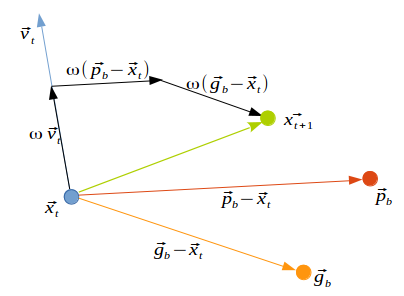
\includegraphics[scale=0.8]{tresc/pics/psoRuch.png}
\caption{Wizualizacja ruchu cząstki PSO}
\label{fig:psoWizualizacja}
\end{center}
\end{figure}

W danej iteracji, cząsteczka znajduje się w konkretnym punkcie $x_t$. Zna położenie najlepszej cząsteczki z całej populacji $g_b$, oraz pamięta swoją najlepszą odwiedzoną do tej pory pozycję $p_b$. Osobnik wyzacza wektory przesunięcia względem tych punktów, oraz przemieszczenia z poprzedniej iteracji $v_t$. Każdy z wektorów jest mnożony przez współczynnik inercji $\omega$, a następnie wszystkie wektory są ze sobą składane. Wynikiem złożenia jest nowa pozycja cząsteczki w przestrzeni rozwiązań.

\subsection{Zasada działania algorytmu}
\label{sec:psoDzialanie}
Diagram \ref{fig:psoDiagram} przedstawia pełny mechanizm działania algorytmu. Pierwszym krokiem jest zainicjalizowanie startowej populacji w losowych miejscach przestrzeni rozwiązań. Następnie dla każdego osobnika liczone jest dopasowanie. Jeśli aktualne dopasowanie jest lepsze niż zapamiętane, uaktualniana jest pamiętana pozycja w przestrzeni rozwiązań. W przypadku gdy dopasowanie jest gorsze, zapamiętana informacja pozostaje bez zmian. Kolejnym krokiem jest uaktualnienie informacji najlepszej pozycji z całej populacji. Posiadając wszystkie informacje, cząsteczka wyznacza swoją prędkość w danej iteracji, a następnie przemieszcza się zgodnie z nią w przestrzeni rozwiązań. Aż do spełnienia warunku stopu (uzyskanie pożądanego dopasowania lub osiągnięcia limitu iteracji), cząsteczki ponownie wyliczają sewoje dopasowanie i powtarzają cały cykl.

\begin{figure}[H]
\begin{center} 
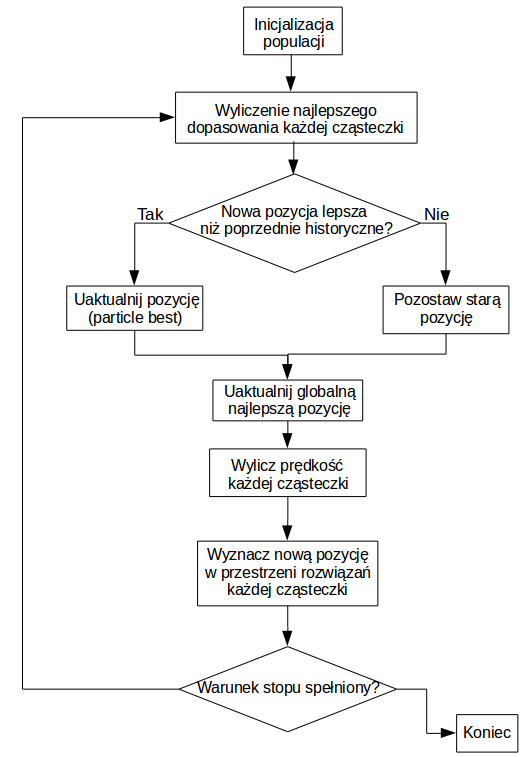
\includegraphics[scale=0.55]{tresc/pics/psoDiagram.png}
\caption{Diagram blokowy algorytmu PSO}
\label{fig:psoDiagram}
\end{center}
\end{figure}


\section{Modyfikacje algorytmu roju cząstek}
\label{sec:psoModyfikacje}
W paragrafie \ref{sec:psoOpis} została przedstawiona podstawowa, najprostsza wersja algorytmu roju cząstek. Istnieje szereg rozszerzeń i modyfikacji algorytmu, które powodują zwiększenie jego dokładności i skuteczności.



\subsection{Rozszerzenie wiedzy cząstek}
\label{sec:psoSasiedztwo}
Rozszerzając wiedzę jednostek o dodatkowe informacje o otoczeniu, często okazuje się, że zwiększa się dokładność jak i prędkość w jakiej otrzymywany jest satysfakcjonujący wynik. Jednym ze sposobów, jest dodanie wiedzy o położeniu najlepszej cząsteczki w pewnym otoczeniu danego osobnika \cite{PSOneighbourhood}. Dołożenie takiego parametru, pociąga za sobą zmianę wyliczania ruchu cząstki (rys. \ref{fig:psoWizualizacja}) o dodatkowy wektor. Podejście takie zwiększa skupienie cząsteczek i pozwala na dokładniejsze przeszukiwanie przestrzeni rozwiązań w danym zakresie. 


\subsection{Dodanie losowej składowej}
\label{sec:psoLosowa}
Uwzględnienie podczas ruchu cząstki dodatkowego składowego wektora, którego wartość oraz kierunek generowana jest losowo, daje możliwość pozbycia się pewnych potencjalnych problemów \cite{PSOrandom}. Cząstki które poruszają się w sposób opisany w rozdziale \ref{sec:psoPrzemieszczenie}, oraz te rozszerzone o informacje o sąsiedztwie, obarczone są ryzykiem wpadania w lokalne ekstrema. Dodając losową składową, wymuszany jest ruch często oddalający osobnika od roju, co może skutkować wyskoczeniem z lokalnego ekstremum i dalsze przeszuiwanie przestrzeni rozwiązań w celu znalezienia ekstremum globalnego.


\subsection{Nadawanie wag parametrom}
\label{sec:psoWagi}
Podstawowa wersja algorytmu roju cząstek zakłada jednakową wagę każdego z wektorów podczas wyliczania nowej pozycji cząstki. Modyfikacja wprowadzająca dla każdego wektora parametr definiujący jego wagę, pozwala na lepsze dostosowanie algorytmu dla danego problemu \cite{PSOparams}.


\subsection{Zmiana prędkości ruchu}
\label{sec:psoPredkosc}
Algorytm roju cząstek w swojej pierwotnej wersji nie zakładał zmiany prędkości osobników w czasie. Rozszerzenie dające możliwość manipulowania współczynnikiem inercji $\omega$ na przestrzeni kolejnych iteracji pozwala na uniknięcie potencjalnego "przeskakiwania" poprawnego rozwiązania przez członków populacji. Wersja podstawowa niesie za sobą ryzyka, że po pewnej ilości iteracji cząsteczki będą krążyły wokół ekstremum, jednak długość wektora będzie zbyt duża, aby udało się im "trafić" w rozwiązanie. Zmniejszanie współczynnika $\omega$ wraz z kolejnymi iteracjami pozwoli cząstkom dokładniej przeszukać dany zakres, jednocześnie utrzymując szeroki zasięg przeszukiwań na początku działania algorytmu \cite{PSOvelocity}.

